\chapter{Alcenos e alcinos: adições eletrofílicas}\label{ch:b1:electrophilic-additions}

Agite um alceno com água de bromo alaranjada e a cor desaparece em
segundos: o mais antigo teste de uma ligação dupla carbono--carbono. Por
trás dele há um mecanismo. Os elétrons $\pi$ da ligação dupla, menos
presos que os elétrons $\sigma$ e expostos acima e abaixo do plano da
molécula, atacam um reagente pobre em elétrons; o cátion formado captura
em seguida um \omterm{def:b1:electronic-effects:nucleophile}{nucleófilo}. As mesmas duas etapas adicionam haletos de
hidrogênio, água e halogênios aos alcenos, decidem qual carbono recebe
qual parte do reagente e fixam a estereoquímica do produto. Este capítulo
as desenvolve, com a regra que um químico do século XIX tirou da
observação e o \omterm{def:b1:electronic-effects:intermediates}{carbocátion} que a explica.

\begin{recall}
Os \omterm{def:b1:electronic-effects:intermediates}{carbocátions}, sua estabilidade e as \omterm{def:b1:electronic-effects:curly-arrow}{setas curvas} (\cref{ch:b1:electronic-effects});
o postulado de Hammond (\cref{prop:b1:elementary-steps:hammond}); os
descritores $Z$/$E$, \cip{R}/\cip{S}, os \omterm{def:b1:stereochemistry-in-depth:enantiomers}{compostos meso} e as \omterm{def:b1:stereochemistry-in-depth:enantiomers}{misturas
racêmicas} (\cref{ch:b1:stereochemistry-in-depth}). O Livro 1 (ano 12)
listou as adições aos alcenos sem os seus mecanismos.
\end{recall}

\section{A ligação \texorpdfstring{$\pi$}{pi} como nucleófilo}

\begin{definition}[Adição eletrofílica]\label{def:b1:electrophilic-additions:electrophilic-addition}
Uma \emph{adição eletrofílica}\index{adicao eletrofilica@adição eletrofílica} a uma
ligação múltipla é uma adição cuja primeira etapa é o ataque dos
elétrons $\pi$ a um \omterm{def:b1:electronic-effects:nucleophile}{eletrófilo} E: forma-se um cátion, que captura em
seguida um \omterm{def:b1:electronic-effects:nucleophile}{nucleófilo} Nu, de modo que E e Nu terminam nos dois carbonos
da antiga ligação dupla.
\end{definition}

A ligação $\pi$ é a mais fraca das duas ligações de C=C (\cref{ch:b1:lewis-resonance-vsepr}),
e seus elétrons ficam longe dos núcleos, acima e abaixo do plano: os
alcenos são \omterm{def:b1:electronic-effects:nucleophile}{nucleófilos}, e reagem com ácidos, halogênios e outros
\omterm{def:b1:electronic-effects:nucleophile}{eletrófilos} que deixam intactos os alcanos saturados.

\section{Adição de haletos de hidrogênio: a regra de Markovnikov}

\begin{omfigure}
\setchemfig{atom sep=2.1em}
\schemestart
\chemfig{H_3C-[:30]@{c2}CH=[@{pi},,,,]@{c1}CH_2}
\+
\chemfig{@{h}H-[@{hb}]@{br}Br}
\arrow{->}
\chemfig{H_3C-[:30]CH^{+}-[:-30]CH_3}
\+
\chemfig{Br^{-}}
\arrow{->}
\chemfig{H_3C-[:30]CH(-[2]Br)-[:-30]CH_3}
\schemestop
\chemmove{\draw[->, thick, shorten <=2pt, shorten >=2pt](pi) .. controls +(90:7mm) and +(110:7mm) .. (h);
          \draw[->, thick, shorten <=2pt, shorten >=2pt](hb) .. controls +(-90:5mm) and +(-90:5mm) .. (br);}

{\small Adição de brometo de hidrogênio ao propeno. O par $\pi$ capta o
próton, no carbono terminal, dando o \omterm{def:b1:electronic-effects:intermediates}{carbocátion} secundário; o íon
brometo se adiciona a ele: 2-bromopropano.}
\end{omfigure}

\begin{proposition}[Regra de Markovnikov]\label{prop:b1:electrophilic-additions:markovnikov}
Na adição de HX a um alceno assimétrico, o hidrogênio vai para o carbono
da ligação dupla que já leva mais hidrogênios
(\emph{regra de Markovnikov}\index{regra de Markovnikov}). Em forma moderna:
o \omterm{def:b1:electronic-effects:nucleophile}{eletrófilo} se adiciona de modo a dar o \omterm{def:b1:electronic-effects:intermediates}{carbocátion} mais estável.
\end{proposition}

\begin{proof}
A transferência de próton é a \omterm{def:b1:elementary-steps:rds}{etapa determinante}, endotérmica, e termina
em um \omterm{def:b1:electronic-effects:intermediates}{carbocátion}. Pelo postulado de Hammond
(\cref{prop:b1:elementary-steps:hammond}), seu \omterm{def:b1:elementary-steps:energy-profile}{estado de transição} se
parece com o \omterm{def:b1:electronic-effects:intermediates}{carbocátion}, de modo que o caminho para o \omterm{def:b1:electronic-effects:intermediates}{carbocátion} mais
estável tem a barreira mais baixa e é muito mais rápido. Pôr o próton no
carbono com mais hidrogênios deixa a carga no carbono com mais grupos
alquila, o cátion mais estável (\cref{prop:b1:electronic-effects:carbocation-order}).
\end{proof}

\begin{omfigure}
\begin{tikzpicture}
\begin{axis}[
  width=0.78\linewidth, height=5.0cm, xmin=0, xmax=10, ymin=-45, ymax=125,
  axis x line=bottom, axis y line=left, xlabel={coordenada de reação},
  ylabel={energia}, xtick=\empty, ytick=\empty, label style={font=\small},
  legend style={font=\scriptsize, draw=none, at={(0.5,-0.30)}, anchor=north}, legend columns=2]
\addplot[omThm, thick, dashed] table[x=x, y=E] {figdata/out/bachelor-1-energy-profiles-primary.dat};
\addplot[omDef, very thick] table[x=x, y=E] {figdata/out/bachelor-1-energy-profiles-secondary.dat};
\legend{via cátion primário, via cátion secundário}
\node[font=\scriptsize, anchor=south] at (axis cs:5,103) {\ce{CH3CH2CH2+}};
\draw[omThm, densely dotted] (axis cs:5,103) -- (axis cs:5,87);
\node[font=\scriptsize, anchor=north] at (axis cs:5,43) {\ce{CH3CH+CH3}};
\node[font=\scriptsize, anchor=north west] at (axis cs:0.1,-3) {propeno + HBr};
\end{axis}
\end{tikzpicture}

{\small \omterm{def:b1:elementary-steps:energy-profile}{Perfis de energia} esquemáticos das duas adições possíveis de HBr
ao propeno. O \omterm{def:b1:electronic-effects:intermediates}{carbocátion} secundário, mais estável, fica mais baixo, e,
pelo postulado de Hammond, também o \omterm{def:b1:elementary-steps:energy-profile}{estado de transição} que leva a ele:
o produto de Markovnikov se forma muito mais depressa.}
\end{omfigure}

\begin{definition}[Rearranjo de carbocátion]\label{def:b1:electrophilic-additions:rearrangement}
Um \emph{rearranjo de carbocátion}\index{rearranjo de carbocation@rearranjo de carbocátion} é a
migração, dentro de um \omterm{def:b1:electronic-effects:intermediates}{carbocátion}, de um átomo de hidrogênio ou de um
grupo alquila com seu \omterm{def:b1:lewis-resonance-vsepr:lewis}{par ligante} para o carbono catiônico vizinho,
dando um \omterm{def:b1:electronic-effects:intermediates}{carbocátion} mais estável (um deslocamento 1,2).
\end{definition}

\begin{example}[Um deslocamento de metila]\label{ex:b1:electrophilic-additions:shift}
O 3,3-dimetilbut-1-eno e o cloreto de hidrogênio dão um \omterm{def:b1:electronic-effects:intermediates}{carbocátion}
secundário vizinho de um carbono quaternário; um grupo metila migra com
seu par, formando um cátion terciário. O produto principal é o
2-cloro-2,3-dimetilbutano, cujo esqueleto difere do do alceno; o
3-cloro-2,2-dimetilbutano é minoritário.
\end{example}

\begin{omfigure}
\setchemfig{atom sep=2em}
\schemestart
\chemfig{C(-[2]CH_3)(-[6]CH_3)(-[4]H_3C)-CH^{+}-CH_3}
\arrow{->[migração 1,2]}[,1.5]
\chemfig{C^{+}(-[2]CH_3)(-[4]H_3C)-CH(-[6]CH_3)-CH_3}
\arrow{->[\ce{Cl-}]}
\chemfig{C(-[2]CH_3)(-[6]Cl)(-[4]H_3C)-CH(-[6]CH_3)-CH_3}
\schemestop
\par\vspace{6pt}

{\small Rearranjo do cátion 3,3-dimetilbutan-2-ila: um grupo metila migra
para o carbono catiônico, transformando um cátion secundário em um
terciário, capturado pelo cloreto.}
\end{omfigure}

\section{Adição de água}

\begin{definition}[Hidratação de um alceno]\label{def:b1:electrophilic-additions:hydration}
A \emph{hidratação}\index{hidratacao@hidratação} de um alceno é a adição
de água, catalisada por um \omterm{def:b1:predominant-reaction:strong-acid}{ácido forte}, que dá um álcool: o inverso da
\omterm{def:b1:alcohol-activation:dehydration}{desidratação} do \cref{ch:b1:alcohol-activation}.
\end{definition}

O mecanismo é o de HX com a água como \omterm{def:b1:electronic-effects:nucleophile}{nucleófilo}: protonação
(Markovnikov), captura do \omterm{def:b1:electronic-effects:intermediates}{carbocátion} pela água, perda de um próton do
íon oxônio. O propeno dá propan-2-ol, o 2-metilpropeno dá
2-metilpropan-2-ol. \omterm{def:b1:electrophilic-additions:hydration}{Hidratação} e \omterm{def:b1:alcohol-activation:dehydration}{desidratação} são o mesmo equilíbrio,
\ce{C3H6 + H2O <=> C3H8O}; ácido aquoso diluído e temperatura baixa
favorecem o álcool, ácido concentrado, calor e remoção do alceno
favorecem o alceno (\cref{ch:b1:extent-q-and-k}).

\section{Adição de halogênios: íons halônio e adição anti}

\begin{definition}[Íon halônio, adição anti e adição sin]\label{def:b1:electrophilic-additions:halonium}
Na adição de \ce{Br2} ou \ce{Cl2}, o par $\pi$ ataca um átomo de halogênio
enquanto um \omterm{def:b1:lewis-resonance-vsepr:lewis}{par não ligante} desse átomo se liga ao segundo carbono:
forma-se um \emph{íon halônio}\index{ion halonio@íon halônio} cíclico de
três átomos, e o outro halogênio sai como haleto. Uma adição em que os
dois novos grupos terminam em faces opostas da antiga ligação dupla é uma
\emph{adição anti}\index{adicao anti@adição anti}; na mesma face, uma
\emph{adição sin}\index{adicao sin@adição sin}.
\end{definition}

\begin{proposition}[A adição de halogênio é anti]\label{prop:b1:electrophilic-additions:anti-addition}
A adição de bromo a um alceno é uma \omterm{def:b1:electrophilic-additions:halonium}{adição anti}: o \cip{E}-but-2-eno dá o
meso-2,3-dibromobutano, e o \cip{Z}-but-2-eno dá a \omterm{def:b1:stereochemistry-in-depth:enantiomers}{mistura racêmica} de
\cip{2R,3R}- e \cip{2S,3S}-2,3-dibromobutano.
\end{proposition}

\begin{proof}
O íon bromônio faz uma ponte sobre uma face da antiga ligação dupla; o
brometo só pode atacar um carbono pela outra face, abrindo o anel como
uma SN2 com inversão nesse carbono. Os dois bromos terminam em faces
opostas. Para o \cip{E}-but-2-eno, o ataque a qualquer um dos carbonos dá
o mesmo produto, em que os dois estereocentros são imagens especulares
um do outro: \cip{2R,3S}, meso. Para o \cip{Z}-but-2-eno, o ataque a um
carbono dá \cip{2R,3R}, ao outro \cip{2S,3S}, com igual probabilidade:
uma \omterm{def:b1:stereochemistry-in-depth:enantiomers}{mistura racêmica}. A prova pelo desenho é o \cref{exo:b1:electrophilic-additions:10}.
\end{proof}

\begin{omfigure}
\begin{tikzpicture}[font=\small, >={Stealth}]
  % íon bromônio a partir do (E)-but-2-eno
  \coordinate (a) at (0,0); \coordinate (b) at (1.4,0);
  \draw[thick] (a) -- (b);
  \node[circle, fill=white, inner sep=1pt] (br) at (0.7,1.0) {\ce{Br+}};
  \draw[thick] (a) -- (br.south west) (b) -- (br.south east);
  \draw[thick] (a) -- ++(-0.8,0.35) node[left] {H};
  \draw[thick] (a) -- ++(-0.6,-0.6) node[below left] {\ce{CH3}};
  \draw[thick] (b) -- ++(0.8,0.35) node[right] {\ce{CH3}};
  \draw[thick] (b) -- ++(0.6,-0.6) node[below right] {H};
  \node (bm) at (0.7,-1.6) {\ce{Br-}};
  \draw[->, thick, omThm] (bm) to[bend left=25] (0.12,-0.12);
  \node[align=center] at (0.7,-2.4) {ataque pela face oposta à ponte};
  \draw[->, thick] (3.3,0) -- (4.4,0);
  \node[align=center] at (6.2,0) {\chemfig{C(-[:150]H_3C)(<[:210]H)(<:[2]Br)-C(<:[:30]H)(-[:-30]CH_3)(<[6]Br)}};
  \node at (6.2,-1.8) {produto anti: meso-2,3-dibromobutano};
\end{tikzpicture}

{\small O íon bromônio formado a partir do \cip{E}-but-2-eno, e sua
abertura pelo brometo pela face oposta (\omterm{def:b1:electrophilic-additions:halonium}{adição anti}). O produto tem dois
estereocentros de descritores opostos e um plano de simetria interno em
uma \omterm{def:b1:stereochemistry-in-depth:isomers}{conformação} adequada: o \omterm{def:b1:stereochemistry-in-depth:enantiomers}{composto meso}, \cip{2R,3S}.}
\end{omfigure}

\begin{inthelab}[Água de bromo]
O bromo é um líquido denso, volátil, muito tóxico e corrosivo. O teste de
insaturação usa água de bromo diluída (ou uma solução comercial de um
\omterm{def:b1:complexation:complex}{complexo} de bromo) em capela, algumas gotas de cada vez; o
desaparecimento da cor alaranjada sinaliza uma adição. Em água, o íon
bromônio também é capturado pela água, e uma bromo-hidrina se forma ao
lado do dibrometo.
\end{inthelab}

\section{Alcinos: adições e acetiletos}

Os alcinos adicionam HX e \ce{X2} duas vezes, cada etapa como para os
alcenos (Markovnikov para HX). Sua \omterm{def:b1:electrophilic-additions:hydration}{hidratação}, catalisada por ácido e um
sal de mercúrio(II), não dá o álcool insaturado esperado, mas uma cetona:
um enol se rearranja de imediato no composto carbonílico, um processo
estudado no volume do 2.º~ano.

\begin{definition}[Alcino terminal, acetileto]\label{def:b1:electrophilic-additions:acetylide}
Um \emph{alcino terminal}\index{alcino terminal} \ce{R-C#C-H} tem sua
ligação tripla na extremidade da cadeia. Uma \omterm{def:b1:predominant-reaction:strong-acid}{base forte} (amideto de
sódio) remove seu hidrogênio, dando o \emph{íon acetileto}\index{ion acetileto@íon acetileto}
\ce{R-C#C-}, um bom \omterm{def:b1:electronic-effects:nucleophile}{nucleófilo} de carbono.
\end{definition}

\begin{proposition}[Acidez dos alcinos terminais]\label{prop:b1:electrophilic-additions:acetylide-acidity}
A ligação C--H de um \omterm{def:b1:electrophilic-additions:acetylide}{alcino terminal} é muito mais ácida que as dos
alcenos e dos alcanos, embora ainda muito menos ácida que a água: os
acetiletos são formados com íons amideto, não com hidróxido, e são
destruídos pela água.
\end{proposition}

\begin{proof}
No \omterm{def:b1:electrophilic-additions:acetylide}{íon acetileto}, o \omterm{def:b1:lewis-resonance-vsepr:lewis}{par não ligante} ocupa um orbital com metade de
caráter \textit{s} (carbono \textit{sp}), mantido mais perto do núcleo que
os orbitais dos \omterm{def:b1:electronic-effects:intermediates}{carbânions} \textit{sp}$^2$ ou \textit{sp}$^3$: ele é mais
estável, e seu ácido conjugado, mais forte. Ele continua sendo uma base
muito mais forte que o hidróxido, de modo que a água o protona.
\end{proof}

Um acetileto ataca um haloalcano primário por SN2 (uma nova ligação C--C,
\ce{R-C#C-} + $\mathrm{R'Br}$) ou se adiciona a uma carbonila como um
\omterm{def:b1:organomagnesium:organometallic}{reagente de Grignard}: outra maneira de construir esqueletos carbônicos.

\begin{method}[Prever uma adição]\label{met:b1:electrophilic-additions:predict-addition}
\begin{enumerate}
  \item Identifique o \omterm{def:b1:electronic-effects:nucleophile}{eletrófilo} (\ce{H+}, \ce{Br2}) e o \omterm{def:b1:electronic-effects:nucleophile}{nucleófilo} que
        virá em seguida (\ce{X-}, água, o haleto).
  \item Para \ce{H+}: adicione-o ao carbono que dá o \omterm{def:b1:electronic-effects:intermediates}{carbocátion} mais
        estável (Markovnikov); verifique um possível deslocamento 1,2.
  \item Para \ce{X2}: forme a ponte do \omterm{def:b1:electrophilic-additions:halonium}{íon halônio} e abra-o pela face
        oposta (anti); desenhe os dois ataques possíveis e compare os
        produtos (meso ou racêmico).
  \item Com água presente, espere também o álcool (ou a
        halo-hidrina).
\end{enumerate}
\end{method}

\begin{history}[Vladimir Markovnikov]
\begin{minipage}[t]{0.2\linewidth}\vspace{0pt}
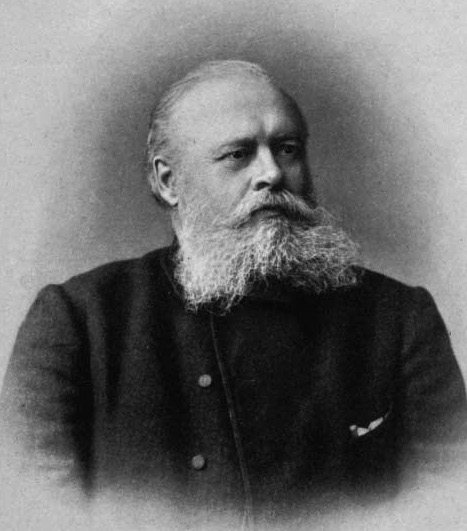
\includegraphics[width=\linewidth]{images/book2/markovnikov.jpg}
\end{minipage}\hfill
\begin{minipage}[t]{0.76\linewidth}\vspace{0pt}
Vladimir Markovnikov enunciou sua regra no século XIX, a partir dos
produtos que ele e outros observavam, muito antes de existirem
\omterm{def:b1:electronic-effects:intermediates}{carbocátions} ou \omterm{def:b1:electronic-effects:curly-arrow}{setas curvas}: uma regularidade da natureza, registrada
antes que pudesse ser explicada. Seu enunciado moderno pela estabilidade
dos \omterm{def:b1:electronic-effects:intermediates}{carbocátions} mostra o que um mecanismo acrescenta a uma regra
empírica: ele diz quando a regra deve falhar.
(Retrato de um obituário publicado em 1905, domínio público,
Wikimedia Commons.)
\end{minipage}
\end{history}

\section{Exercícios}

\begin{exercise}[$\star$]\label{exo:b1:electrophilic-additions:1}
Dê o produto principal de: propeno + HCl; 2-metilpropeno + HBr;
1-metilciclo-hexeno + HBr; but-2-ino + um equivalente de HCl.
\end{exercise}

\begin{exercise}[$\star$]\label{exo:b1:electrophilic-additions:2}
Escreva os produtos do bromo com o eteno, o ciclo-hexeno e o propeno.
Dê seus nomes.
\end{exercise}

\begin{exercise}[$\star$]\label{exo:b1:electrophilic-additions:3}
Que álcool a \omterm{def:b1:electrophilic-additions:hydration}{hidratação} catalisada por ácido de cada alceno dá:
propeno, 2-metilpropeno, metilenociclo-hexano?
\end{exercise}

\begin{exercise}[$\star$]\label{exo:b1:electrophilic-additions:4}
Quais destes compostos reagem com o amideto de sódio: propino, but-2-ino,
propeno, etanol? Escreva as reações.
\end{exercise}

\begin{exercise}[$\star\star$]\label{exo:b1:electrophilic-additions:5}
Escreva o mecanismo completo da \omterm{def:b1:electrophilic-additions:hydration}{hidratação} do 2-metilpropeno com \omterm{def:b1:electronic-effects:curly-arrow}{setas
curvas}, e explique por que a reação inversa é favorecida em ácido
concentrado quente.
\end{exercise}

\begin{exercise}[$\star\star$]\label{exo:b1:electrophilic-additions:6}
Explique com o postulado de Hammond por que o 2-metilpropeno reage com
HCl muito mais depressa que o propeno.
\end{exercise}

\begin{exercise}[$\star\star$]\label{exo:b1:electrophilic-additions:7}
O bromo reage com o ciclo-hexeno. Mostre que o produto é o
\textit{trans}-1,2-dibromociclo-hexano, e diga se ele é \omterm{def:b1:stereochemistry-in-depth:stereocentre}{quiral} e se o
produto é opticamente ativo.
\end{exercise}

\begin{exercise}[$\star\star$]\label{exo:b1:electrophilic-additions:8}
Proponha um mecanismo para a adição de HCl ao 3-metilbut-1-eno que dá
principalmente o 2-cloro-2-metilbutano.
\end{exercise}

\begin{exercise}[$\star\star$]\label{exo:b1:electrophilic-additions:9}
Proponha uma síntese do hex-2-ino a partir do propino e de um
haloalcano, e do 1-fenilbut-2-in-1-ol a partir do propino e do benzaldeído.
\end{exercise}

\begin{exercise}[$\star\star\star$]\label{exo:b1:electrophilic-additions:10}
Prove pelo desenho a estereoquímica da adição de bromo aos dois
but-2-enos: íon bromônio, ataque anti a cada carbono, \omterm{def:b1:stereochemistry-in-depth:representations}{representação de
Cram} dos produtos, descritores. Conte os \omterm{def:b1:stereochemistry-in-depth:isomers}{estereoisômeros} formados em
cada caso.
\end{exercise}

\begin{exercise}[$\star\star\star$]\label{exo:b1:electrophilic-additions:11}
A água de bromo com o propeno dá o 1-bromopropan-2-ol como produto
principal. Explique a regioquímica: por que a água ataca o carbono mais
substituído do íon bromônio?
\end{exercise}

\begin{exercise}[$\star\star\star$]\label{exo:b1:electrophilic-additions:12}
Um hidrocarboneto \ce{C5H10} descora a água de bromo e adiciona HBr dando
o 2-bromo-2-metilbutano; sua \omterm{def:b1:electrophilic-additions:hydration}{hidratação} dá o 2-metilbutan-2-ol. Encontre
duas estruturas possíveis e proponha uma maneira de distingui-las.
\end{exercise}

\section{Problema: dois butenos e o bromo}

\begin{problem}[{Problema de fim de semana --- os dois but-2-enos, o
mecanismo do íon bromônio, os dibrometos meso e racêmico, sua rotação
óptica e a massa obtida}]
\label{pb:b1:electrophilic-additions:1}
Um laboratório tem dois frascos de but-2-eno, um \cip{Z} puro, outro
\cip{E} puro, e trata \qty{5.60}{g} de cada um com bromo em
diclorometano. Massas molares (\unit{g/mol}): \ce{C4H8} 56.0, \ce{Br2}
159.8, \ce{C4H8Br2} 215.8.

\medskip
\noindent\textbf{Parte I --- Os dois alcenos.}
\begin{enumerate}
  \item Desenhe o \cip{Z}- e o \cip{E}-but-2-eno e justifique os descritores.
  \item Eles são \omterm{def:b1:stereochemistry-in-depth:isomers}{estereoisômeros}? \omterm{def:b1:stereochemistry-in-depth:enantiomers}{Enantiômeros} ou \omterm{def:b1:stereochemistry-in-depth:enantiomers}{diastereoisômeros}?
  \item Por que eles não se interconvertem à temperatura ambiente?
  \item Qual é o mais estável, e por quê?
  \item Escreva a equação global da adição de bromo.
  \item Quantos estereocentros tem o 2,3-dibromobutano? Quantos
        \omterm{def:b1:stereochemistry-in-depth:isomers}{estereoisômeros} no máximo, e quantos de fato?
\end{enumerate}

\medskip
\noindent\textbf{Parte II --- O mecanismo.}
\begin{enumerate}[resume]
  \item Escreva a formação do íon bromônio com \omterm{def:b1:electronic-effects:curly-arrow}{setas curvas}.
  \item Por que se forma um íon bromônio em ponte e não um \omterm{def:b1:electronic-effects:intermediates}{carbocátion}
        aberto?
  \item Escreva a abertura do íon pelo brometo.
  \item Por que o brometo ataca pela face oposta à ponte?
  \item Que tipo de adição resulta?
  \item Por que o solvente é o diclorometano e não a água?
\end{enumerate}

\medskip
\noindent\textbf{Parte III --- Os produtos.}
\begin{enumerate}[resume]
  \item A partir do \cip{E}-but-2-eno: desenhe o produto do ataque em C2 e
        dê os descritores de C2 e C3.
  \item O mesmo para o ataque em C3. Compare.
  \item Mostre que o produto é meso.
  \item A partir do \cip{Z}-but-2-eno: desenhe os dois produtos e seus
        descritores.
  \item Em que proporções eles se formam? Dê o nome da mistura.
  \item A reação é estereoespecífica? Justifique.
\end{enumerate}

\medskip
\noindent\textbf{Parte IV --- Rotação e massa.}
\begin{enumerate}[resume]
  \item Que rotação óptica o produto do alceno \cip{Z} apresenta?
  \item Calcule a quantidade de matéria de cada alceno.
  \item Calcule a massa de dibrometo esperada a partir de cada um com
        \qty{85}{\percent} de \omterm{def:b1:extent-q-and-k:fractional-extent}{rendimento}.
  \item Indique o \omterm{def:b1:stereochemistry-in-depth:optical-activity}{poder rotatório específico} do dibrometo obtido a partir
        do \cip{E}-but-2-eno, e a massa obtida dele.
\end{enumerate}
\end{problem}
